\documentclass[a4]{article}

\usepackage[left=2cm,right=2cm,top=2cm,bottom=2cm]{geometry} 

\usepackage[utf8]{inputenc}   % otra alternativa para los caracteres acentuados y la "ñ"
\usepackage[           spanish % para poder usar el español
                      ,es-tabla % para los captions de las tablas
                       ]{babel}   
\decimalpoint %para usar el punto decimal en vez de coma para los números con decimales

\usepackage{beton}
\usepackage[T1]{fontenc}

\usepackage{parskip}
\usepackage{xcolor}

\usepackage{caption}

\usepackage{enumerate} % paquete para poder personalizar fácilmente la apariencia de las listas enumerativas

\usepackage{graphicx} % figuras
\usepackage{subfigure} % subfiguras

\usepackage{amsfonts}
\usepackage{amsmath}

\usepackage{chngcntr}

\counterwithin*{equation}{section}

\definecolor{gris}{RGB}{220,220,220}
	
\usepackage{float} % para controlar la situación de los entornos flotantes

\restylefloat{figure}
\restylefloat{table} 
\setlength{\parindent}{0mm}


\usepackage[bookmarks=true,
            bookmarksnumbered=false, % true means bookmarks in 
                                     % left window are numbered
            bookmarksopen=false,     % true means only level 1
                                     % are displayed.
            colorlinks=true,
            allcolors=blue]{hyperref}
\definecolor{webblue}{rgb}{0, 0, 0.5}  % less intense blue


\title{Ejercicios de química y ecuación de ondas}

\author{David Cabezas Berrido}

\date{\vspace{-4mm}}

\begin{document}
\maketitle

\section{Ejercicio de química}

Consideramos la siguiente reacción química: $A+B\rightarrow C$

Ecuación de velocidad de reacción: $v=k[A]^\alpha [B]^\beta$.
En este caso tenemos $k=1$, $\alpha=1$, $\beta=2$.

Vamos a denotar como $a(t)$ a la concentración del reactivo $A$ en el
instante $t$. Análogamente, denotaremos $b(t)$ y $c(t)$ a las
concentraciones de los reactivos $B$ y $C$ respectivamente, en el
instante $t$. Las concentraciones se miden en moles por litro
($mol/L$).

Suponemos que estamos en un recipiente de volumen constante 1 litro,
por lo que las concentraciones de cada reactivo ($a$, $b$ y $c$)
equivalen al número de moles.

\textbf{a)}
Partimos de $0.8\ mol/L$ de $A$, $0.6\ mol/L$ de $B$ y nada de
producto ($C$), esto se traduce en que $a(0)=0.8$, $b(0)=0.6$ y
$c(0)=0$.

Primero se nos pide determinar la ecuación diferencial para la
cantidad de producto ($c$) y usar un integrador numérico de ecuaciones
diferenciales para calcular la cantidad de producto tras 20 segundos
($c(20)$) y tras mucho tiempo
\Big($\lim\limits_{t\to +\infty}c(t)$\Big).

\vspace{6mm}

Intuitivamente: \\
En la reacción, se gastan un mol de $A$ y un mol de $B$ para producir
un mol de $C$. Hay concentración de $A$ suficiente para producir $0.8$
moles de $C$ y concentración de $B$ para producir $0.6$ moles de
$C$. Por tanto $B$ es el reactivo limitante, que se agotará por
completo, produciéndose $0.6$ moles de $C$ y sobrando $0.2$ moles de
$A$. Veamos esto de forma analítica.

Partimos de la ecuación de velocidad media de reacción, que estudia la
variación de concentración de reactivo en un incremento de tiempo.
\begin{equation}
  \label{eq:v-media}
  -\frac{a(t)-a(t_0)}{t-t_0}=-\frac{b(t)-b(t_0)}{t-t_0}=\frac{c(t)-c(t_0)}{t-t_0}
\end{equation}

Haciendo el incremento de tiempo tender a 0, obtenemos la
derivada. Por tanto $-a'(t)=-b'(t)=c'(t)$. Y es a esta cantidad a la
que llamaremos $v(t)=c'(t)$, que sabemos que cumple $v(t)=a(t)b(t)^2$.

Por otra parte, tomando en (\ref{eq:v-media}) $t_0=0$ y simplificando,
obtenemos
\begin{equation} \label{eq:acbc}
  -(a(t)-0.8)=-(b(t)-0.6)=c(t)-0\quad \Longrightarrow\quad
  a(t)=0.8-c(t),\quad b(t)=0.6-c(t)
\end{equation}
y sustituyendo en la ecuación de la velocidad de reacción, obtenemos
la ecuación diferencial que modela la cantidad de producto
\begin{equation}
  \label{eq:c-a}
  c'(t)=\big(0.8-c(t)\big)\big(0.6-c(t)\big)^2\ ;\qquad c(0)=0
\end{equation}

Para estimar $c(20)$, usaré el método de Runge-Kutta de orden 4,
tomando 100000 puntos en el intervalo $[0,20]$. Obtengo
\[c(20)\approx 0.4956\ \ \text{ moles}\]

Podemos calcular analíticamente $\lim\limits_{t\to +\infty}c(t)$.

La ecuación diferencial (\ref{eq:c-a}) es
$c'=f(c)=\big(0.8-c\big)\big(0.6-c\big)^2$, es autónoma y claramente
tiene a $c=0.8$ y $c=0.6$ como puntos de quilibrio. Podemos estudiar
su comportamiento en el infinito bajo la condición inicial $c(0)=0$.

$f$ es de esta forma
\begin{figure}[H]
  \centering
  \subfigure[Gráfica de $f$]{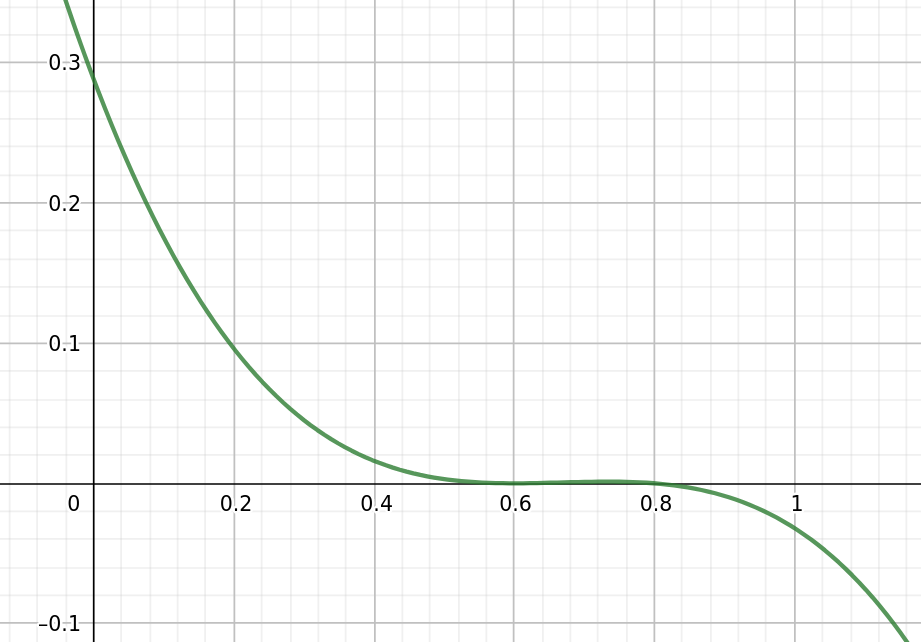
\includegraphics[width=80mm]{imgs/f.png}}
  \subfigure[Zoom de la gráfica]{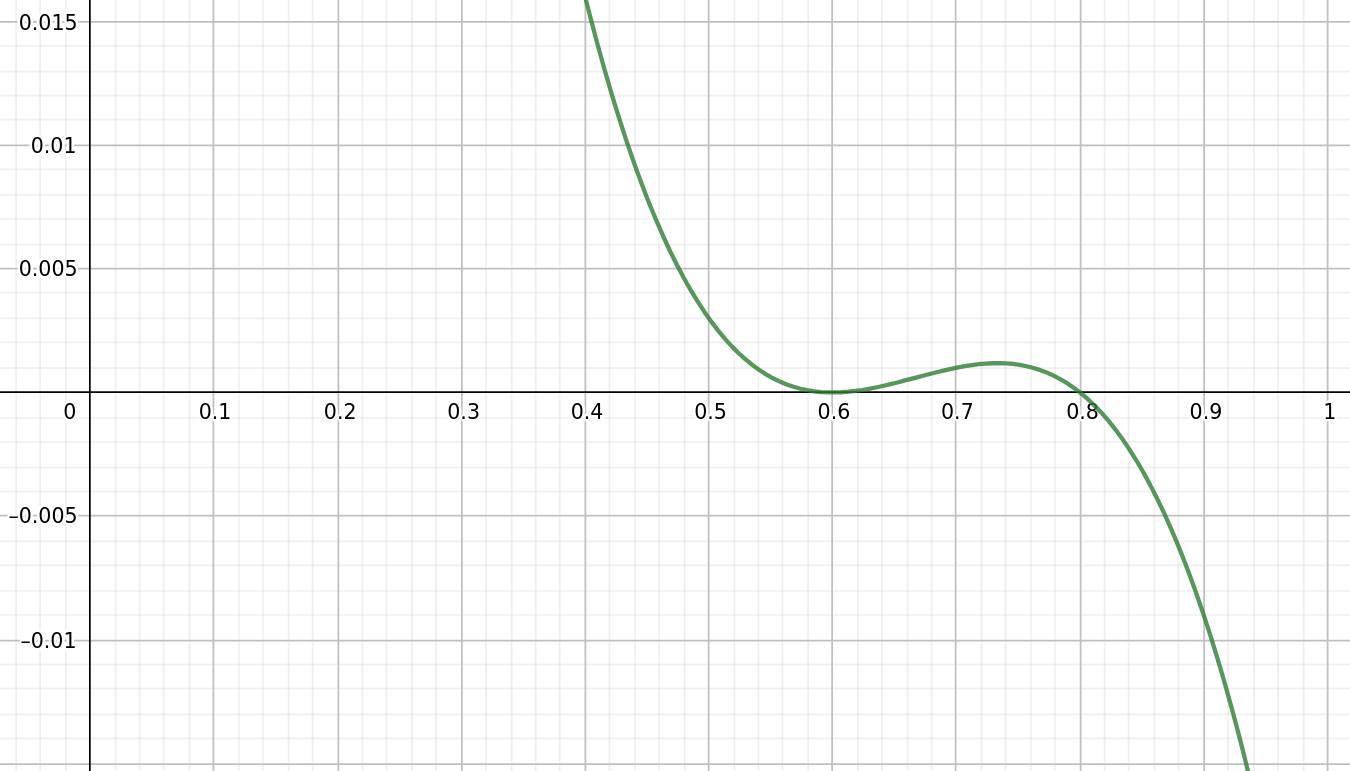
\includegraphics[width=80mm]{imgs/f-zoom.png}}
  \caption{$f(c)=\big(0.8-c\big)\big(0.6-c\big)^2$}
  \label{fig:f}
\end{figure}

Estudiando el signo de $f$ (polinomio de grado 3 con coeficiente líder
negativo), obtenemos el diagrama de fases: \vspace{-4mm}

\begin{figure}[H]
  \centering
  \subfigure[Instancia correspondiente al 0]{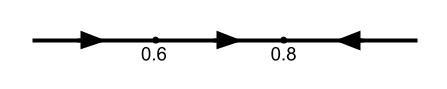
\includegraphics[width=100mm]{imgs/phase.png}}
  \caption{Diagrama de fases y puntos de equilibrio de $f$}
  \label{fig:phase}
\end{figure}
\vspace{-5mm}

Como partimos de $c(0)=0$, estamos en la región de atracción del punto
de equilibrio $c=0.6$, por tanto podemos concluir que
\[\lim\limits_{t\to +\infty}c(t)=0.6\]

Corroboramos nuestra afirmación utilizando el método de Runge-Kutta de
orden 4, tomando 1000000 de puntos en los intervalos $[0,1000]$ y
$[0,10000]$ obtenemos $c(1000)\approx 0.59544$,
$c(10000)\approx 0.59951$.

\begin{figure}[H]
  \centering
  \subfigure[Entre 0 y 20]{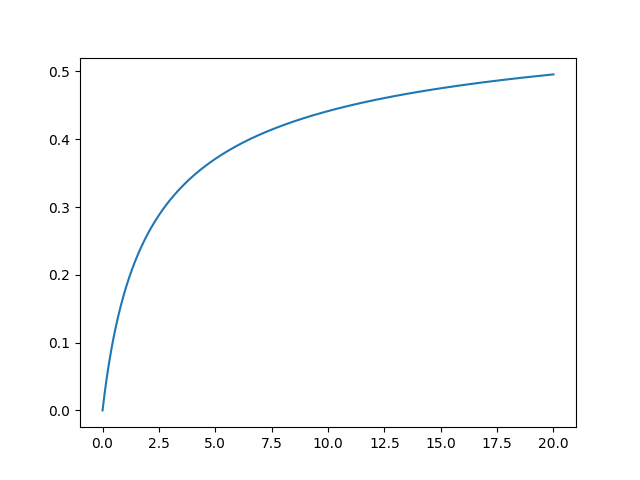
\includegraphics[width=70mm]{imgs/c20.png}}
  \subfigure[Entre 0 y 1000]{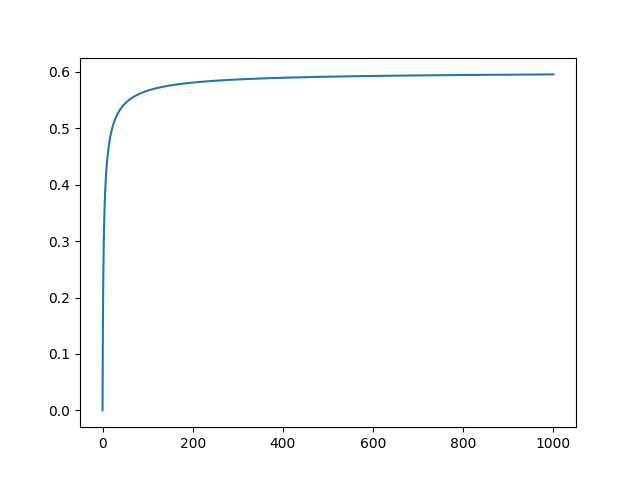
\includegraphics[width=70mm]{imgs/c1000.png}}
  \caption{Aproximación de $c$ por Runge-Kutta}
  \label{fig:runge-kutta}
\end{figure}

\textbf{b)} Ahora $B$ está presente en una concentración ambiente
constante $0.2\ mol/L$, por lo que $B$ no se agota. Por tanto ahora
$A$ es el reactivo limitante, luego se alcanzará una concentración de
$0.8\ mol/L$ del producto.

Tenemos que $b(t)=0.2\ mol/L$ constante, pero la ecuación
(\ref{eq:acbc}) sigue relacionando las concentraciones de los
compuestos $A$ y $C$ correctamente: $a(t)=0.8-c(t)$.

De forma que la ecuación diferencial de la velocidad de reacción queda
ahora
\begin{equation}
  \label{eq:c-b}
  c'(t)=v(t)=a(t)b(t)^2=\big(0.8-c(t)\big)0.2^2\ ;\qquad c(0)=0
\end{equation}
Resolvemos por variables separadas
\[-\log(0.8-c)=\int\frac{dc}{0.8-c}=0.2^2t+q\ \Longrightarrow\
  c(t)=0.8-q'e^{-0.04t}\] Imponiendo $c(0)=0$ ajustamos la constante
de integración, obteniendo la concentración de $C$ en cada instante
\[c(t)=0.8-0.8e^{-0.04t}\] Tras mucho tiempo ($c\to +\infty$), se
alcanzará una concentración de $0.8\ mol/L$ de $C$ como intuíamos. \\
De (\ref{eq:acbc}) despejamos la concentración de $A$
\[a(t)=0.8-c(t)=0.8e^{-0.04t}\] y podemos comprobar que esta
concentración disminuye cada vez más, pero el reactivo $A$ no se llega
a agotarse en tiempo finito.
 
\section{Ejercicio de ecuación de ondas}

Consideramos la ecuación
\begin{equation} \label{eq:ecuacion}
  \begin{cases}
    u_{tt}=u_{xx}+1,\qquad&(t,x)\in [0,+\infty)\times [0,1], \\
    u(t,0)=u(t,1)=0,\qquad &t\in [0,+\infty)
  \end{cases}
\end{equation}

\textbf{a)} Buscamos una solución independiente de $t$, llamémosla
$f(x)$.

Tenemos $f_{tt}=0$ y $f_{xx}=f''$, por tanto la equación diferencial
queda $f''(x)=-1\quad\forall x\in[0,1]$. Por tanto $f$ será una
parábola con coeficiente líder $\frac{-1}{2}$.
\begin{equation} \label{eq:f-ab}
  f(x)=\frac{-1}{2}x^2+ax+b\qquad\forall x\in [0,1]
\end{equation}
Imponemos las condiciones $f(0)=0$ y $f(1)=0$ para obtener $b=0$ y
$\frac{-1}{2}+a=0$, luego sustituyendo en (\ref{eq:f-ab}) obtenemos que
\begin{equation} \label{eq:f}
f(x)=\frac{-1}{2}x^2+\frac{1}{2}x\qquad\forall x\in [0,1]
\end{equation}
es una solución independiente de $t$.

\vspace{4mm}

\textbf{b)} $\phi,\psi:[0,1]\rightarrow\mathbb{R}$. Queremos probar
unicidad de solución de clase 2 para la ecuación (\ref{eq:ecuacion})
con los datos iniciales
\begin{equation} \label{eq:condiciones}
  \begin{cases}
    u(0,x)=\phi(x)\quad\forall x\in [0,1], \\
    u_t(0,x)=\psi(x)\quad\forall x\in [0,1],
  \end{cases}
\end{equation}

Sean $u,v\in C^2([0,+\infty)\times[0,1])$ soluciones de
(\ref{eq:ecuacion}) cumpliendo (\ref{eq:condiciones}). Probaré que
$w=u-v\in C^2([0,+\infty)\times[0,1])$ es constante 0, con lo que
tendremos $u=v$ y por tanto unicidad.

De que $u$ y $v$ satisfacen (\ref{eq:ecuacion}) deducimos
\[w_{tt}-w_{xx}=u_{tt}-v_{tt}-u_{xx}+v_{xx}=1-1=0\]
y
\[w(t,0)=u(t,0)-v(t,0)=0-0=0\]
\[w(t,1)=u(t,1)-v(t,1)=0-0=0\]

Mientras que de $u$ y $v$ cumpliendo (\ref{eq:condiciones}) obtenemos
\[w(0,x)=u(0,x)-v(0,x)=\phi(x)-\phi(x)=0\]
\[w_t(0,x)=u_t(0,x)-v_t(0,x)=\psi(x)-\psi(x)=0\]

Tomando en el \textbf{Teorema 4.1} tanto $\varphi$ como $\psi$ la
función constante 0 (que trivialmente cumple todas las hipótesis del
teorema) obtenemos que el problema
\begin{equation} \label{eq:problema0}
  \begin{cases}
    u_{tt}-u_{xx}=0, \qquad\mbox{en } [0,+\infty)\times [0,1] \\
    u(0,x)=0, \qquad\mbox{en } [0,1] \\
    u_t(0,x)=0, \qquad\mbox{en } [0,1] \\
    u(t,0)=u(t,1)=0, \qquad\mbox{en } [0,+\infty)
  \end{cases}
\end{equation}
tiene solución única (de clase 2).

Hemos comprobado que $w$ es solución del problema y trivialmente la
solución constante 0 también lo es, por tanto deberá suceder $w=0$ y
$u=v$ como queríamos.

\vspace{4mm}

\textbf{c)} Ahora debemos probar que si
$\phi,\psi:[0,1]\rightarrow\mathbb{R}$ son clase 2 y ocurre
$\phi''(0)=0$ o $\phi''(1)=0$, no existe solución de
(\ref{eq:ecuacion}) cumpliendo las condiciones (\ref{eq:condiciones}).

Llegaremos a un absurdo suponiendo que
$u\in C^2([0,+\infty)\times[0,1])$ cumple
(\ref{eq:ecuacion},\ref{eq:condiciones}).

De la segunda condición de (\ref{eq:ecuacion}) obtenemos derivando
respecto a $t$ dos veces que
$u_{tt}(t,0)=u_{tt}(t,1)=0\\ \forall t\in [0,+\infty)$, por tanto
$u_{tt}(0,0)=u_{tt}(0,1)=0$.

Ahora sustituimos en la ecuación para obtener que
$u_{xx}(0,0)=u_{xx}(0,1)=-1$.

Por otra parte, derivando respecto de $x$ dos veces en la primera
igualdad de (\ref{eq:condiciones}) obtenemos \\
$u_{xx}(0,x)=\phi''(x)\quad\forall x \in [0,1]$, por lo que
$-1=u_{xx}(0,0)=\phi''(0)$, $-1=u_{xx}(0,1)=\phi''(1)$. Contradiciendo
la hipótesis.

\vspace{4mm}

\textbf{d)} Tenemos que encontrar
$\phi,\psi:[0,1]\rightarrow\mathbb{R}$ de clase 2 con
$\psi''(0)=\psi''(1)=0$ para las cuales el problema
(\ref{eq:ecuacion},\ref{eq:condiciones}) tenga solución.

Sabemos que la función
\[f(x)=\frac{-1}{2}x^2+\frac{1}{2}x\quad\forall x\in[0,1]\]
satisface (\ref{eq:ecuacion}).

Basta tomar $\phi$ y $\psi$ de clase 2 de forma que $f$ cumpla las
condiciones (\ref{eq:condiciones}) para esas $\phi$ y $\psi$ y además
$\psi''(0)=\psi''(1)=0$. Esto se consigue fácilmente tomando
$\phi(x)=f(x)$ y $\psi(x)=0$ para todo $x$ en $[0,1]$. Claramente son
de clase 2 y $f$ resuelve el problema con esas condiciones iniciales.


\end{document}
